\section{Stochastik}
	\subsection{Zufallsexperimente}
	\subsubsection{Bernoulli-Experiment}
	Ein Bernoulli-Experiment ist ein Zufallsexperiment bei dem es nur zwei mögliche Ergebnisse gibt. Ein Beispiel für ein Bernoulli-Experiment ist der Wurf eines Würfels wo die "1" als Treffer gezählt wird und alle anderen Zahlen als Nieten. Somit sind die zwei Ergen entweder Treffer oder Niete.
	\subsubsection{Laplace-Experiment}
	Bei einem Laplace-Experiment haben alle möglichen Ergebnisse die gleiche Wahrscheinlichkeit. Somit ist ein idealer Würfel ein Laplace-Experiment, da alle Zahlen die gleiche Wahrscheinlichkeit haben gewürfelt zu werden.
	\subsection{Empirische Standardabweichung}
		$$ \overline{s} = \sqrt{p_{1} \cdot (x_{1}-\overline{x})^{2}+p_{2} \cdot (x_{2}-\overline{x})^{2}+p_{3} \cdot (x-\overline{x})^{3}+...} $$
	\subsection{Erwartungswert}
		$$ E(x) = 1 \cdot P(X = 1) + 2 \cdot P(X = 2) + 3 \cdot P(X = 3) + ... $$
	\subsection{Binomialkoeffizient}
$$
\binom{n}{k} =  \frac{n!}{k!\,(n-k)!}
$$

$$
\text{binomPDF: } P(X=Y) = \binom{n}{k} \cdot p^{k} \cdot (1-p)^{n-k}
$$

$$
\text{binomCDF: } P(X\leq Y) = p(x=y) + p(x=y-1) + ... + p(x=y-y)
$$
	\subsection{Vier-Felder-Tafel}
	\begin{center}
	\begin{tabular}{|c|c|c|c|}
	\hline 
	 & $B$ & $\overline{B}$ &  \\ 
	\hline
	$A$ & Wahrscheinlichkeit $AB$ & Wahrscheinlichkeit $A\overline{B}$ & Wahrscheinlichkeit $A$ \\ 
	\hline
	$\overline{A}$ & Wahrscheinlichkeit $\overline{A}B$ & Wahrscheinlichkeit $\overline{AB}$ & Wahrscheinlichkeit $\overline{A}$ \\ 
	\hline
	 & Wahrscheinlichkeit $B$ & Wahrscheinlichkeit $\overline{B}$ & $1$ \\ 
	\hline 
	\end{tabular} 
	\end{center}
	\textbf{Beispiel:} \\
	\\
	\begin{tabular}{|c|c|c|c|}
	\hline 
	 & $B$ & $\overline{B}$ &  \\ 
	\hline
	$A$ & $0.21$ & $0.49$ & $0.7$ \\ 
	\hline
	$\overline{A}$ & $0.06$ & $0.24$ & $0.3$ \\ 
	\hline
	 & $0.27$ & $0.73$ & $1$ \\ 
	\hline 
	\end{tabular}
	\subsection{Sigma-Regeln}
	\subsubsection{Intervalle abschätzen für sigma}
	\begin{center}
	$90\% \rightarrow 1.64 \cdot \sigma$ \\
	$95\% \rightarrow 1.96 \cdot \sigma$ \\
	$99\% \rightarrow 2.58 \cdot \sigma$
	\end{center}
	
	\subsection{Erwartungswert}
	$$ \mu = n \cdot p $$
	\subsection{Standardabweichung}
	$$ \sigma = \sqrt{n \cdot p \cdot (1-p)} $$
	\subsection{Sigma-Regeln andwenden für }
		\begin{enumerate}
			\item Gegeben: n, p
			\item $ \mu = n \cdot p$
			\item $\sigma = \sqrt{n \cdot p \cdot (1-p)}$ $\rightarrow$ Wenn $\sigma >$ 3 ist:
			\begin{enumerate}
				\item $1.64 \cdot \sigma = d$
				\item $\mu -d \leq X \leq \mu + d$
				\item $P(\mu + d (aufrunden) < X <\mu + d (abrunden))$
				\item $P(\mu + d (abrunden) < X <\mu + d (aufrunden))$
				\item Hinweis: Dies kann mit dem binomCDF befehl des CAS berechnet berechnet werden.
				\item Das Ergebnis welches am nächsten über 0.9 liegt ist das bessere Ergebnis
			\end{enumerate}
		\end{enumerate}
	\textbf{Beispiel:}
	\begin{enumerate}
			\item Gegeben: $n = 920$,  $p = 58$
			\item $ \mu = 920 \cdot 0.58 = 533.6$
			\item $\sigma = \sqrt{920 \cdot 0.58 \cdot (0.42)} = 14.9703$ $\rightarrow$ Wenn $\sigma$ > 3 ist:
			\begin{enumerate}
				\item $1.64 \cdot 14.9703 = 24.5513$
				\item $533.6 - 24.5513 \leq X \leq 533.5 + 24.5513 \rightarrow 509.0487 \leq X \leq 558.1513$
				\item $P(510 < X < 558) = 0.8982$
				\item $P(509 < X <559) = 0.9114$
				\item $\rightarrow$ Das richtige Ergebnis ist $P(509 \leq X \leq 559)$
			\end{enumerate}
		\end{enumerate}
	\subsection{Histogramme}
	Histogramme stellen die Wahrscheinlichkeit einer Anzahl von Treffern graphisch dar. Sie sehen Glockenförmig aus wobei die Spitze den Erwartungswert darstellt, welcher die größte Wahrscheinlichkeit besitzt. Die y-Achse gibt die Wahrscheinlichkeit an, während die x-Achse die Anzahl der Ereignisse bzw. Treffer angibt.
	\subsubsection{Beispiel}
	\begin{itemize}
		\item n = 15
		\item p = 0.38
	\end{itemize}
	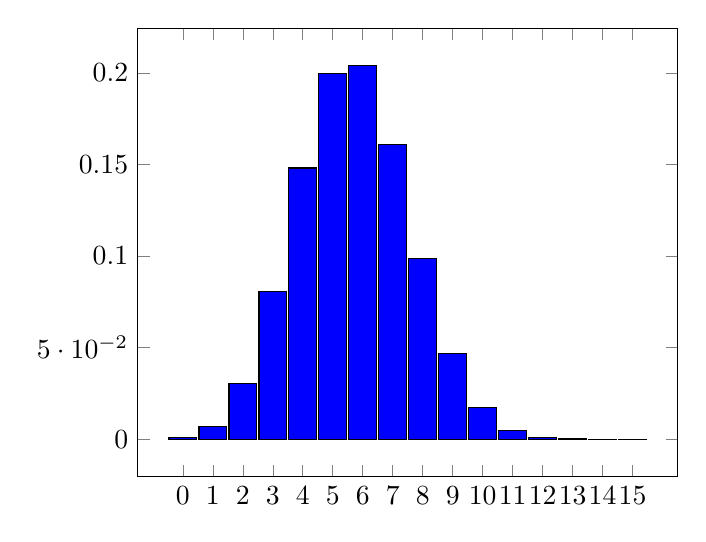
\begin{tikzpicture}
		\begin{axis}[
		symbolic x coords={$0$, $1$, $2$, $3$, $4$, $5$, $6$, $7$, $8$, $9$, $10$, $11$, $12$, $13$, $14$, $15$},
		xtick=data]
		\addplot[ybar,fill=blue] coordinates {
			($0$, 0.000768909705)
			($1$, 0.007069008578)
			($2$, 0.030328327124)
			($3$, 0.080549427953)
			($4$, 0.148107012687)
			($5$, 0.199705584849)
			($6$, 0.20400032861)
			($7$, 0.160756019319)
			($8$, 0.098527882808)
			($9$, 0.046968488937)
			($10$, 0.017272283029)
			($11$, 0.004811926357)
			($12$, 0.000983081729)
			($13$, 0.000139046299)
			($14$, 0.000012174561)
			($15$, 0.00000497455)
		};
		\end{axis}
		\end{tikzpicture}
	\subsubsection{Wahrscheinlichkeiten - y-Achse}
	Die y-Achse gibt die Wahrscheinlichkeit für das eintreten des Ereignisses der x-Achse an.
	
	\subsubsection{Ereignisse/Treffer - x-Achse}
	Die x-Achse gibt die Ereignisse bzw. die Anzahl der Treffer an.
	
	\subsubsection{Erwartungswert im Histogramm}
	Der Erwartungswert im Histogramm wird dadurch gekennzeichnet, dass er die höchste Säule besitzt. Er ist das Produkt aus der Wahrscheinlichkeit und n, also die Anzahl der Möglichkeiten.

	\subsubsection{Histogramme in Klausuren}
	Im Prüfungsteil A der Klausuren können Aufgaben drankommen wo man verschiedene Histogramme vor dem Hintergrund gegebener Kriterien bewerten soll. Bei solchen Aufgaben muss man meistens auf die 3 oben genannten Merkmale eines Histogramms achten. Entweder es gibt Wahrscheinlichkeiten für x-Werte die außerhalb des in der Aufgabenstellung definierten Bereiches liegen. \textbf{ODER} Die Summe aller Wahrscheinlichkeiten im Histogramm sind über 1. Dies ist bei korrekten Histogrammen keine Möglichkeit weshalb das Histogramm falsch ist und den in der Aufgabenstellung beschriebenen Kontext nicht darstellen. \textbf{ODER} Der Erwartungswert liegt nicht an der richtigen Stelle. \textbf{ODER} Eine Kombination von diesen drei Faktoren ist der Fall bzw. in verschiedenen Histogrammen vorhanden. Dies ist keine ausführliche Liste von Merkmalen die man bei Histogrammen analysieren kann, aber diese sind meistens die wichtigsten bei den Aufgaben in Klausuren.